%interaction with it, programs, geometry represenations, datastructures, formats etc., maybe even history if we're overkill
\subsection{History of CAD}
Computer aided design (short: CAD) refers to the process of designing a product using a computer system. Before CAD applications were used, products were constructed using a sketch board. It was a challenge to incorporate changes in the construction drafts as well as to keep documentations up to date; hence, it was no surprise that CAD systems spread rapidly across all design development branches. Computer aided design is now irreplaceable used in architecture, mechanical, electrical and civil engineering.

Depending on the discipline different requirements are set on the virtual model. One may imagine that in a civil engineering model of a building a 2D floor plan is often sufficient; however in the design of a mechanical motor a 3D model is always necessary. Given these circumstances, various CAD software bundles evolved in the different disciplines with completely different modelling approaches. Besides the geometry representation parameters, such as material properties or manufacturing information, are stored. In order to move between different data structures standardized exchange interfaces are commonly used.
\subsection{Geometry representations}
In general, two different ways of describing a geometry are used in CAD systems: constructive solid geometry consisting of a set of primitive forms or storing the boundary of a part assuming that the interior is filled (BREP). Other approaches, such as a complete voxelised geometry are not common due to extensive memory consumption.
\subsubsection{Constructive solid geometry}
\begin{figure}
\centering
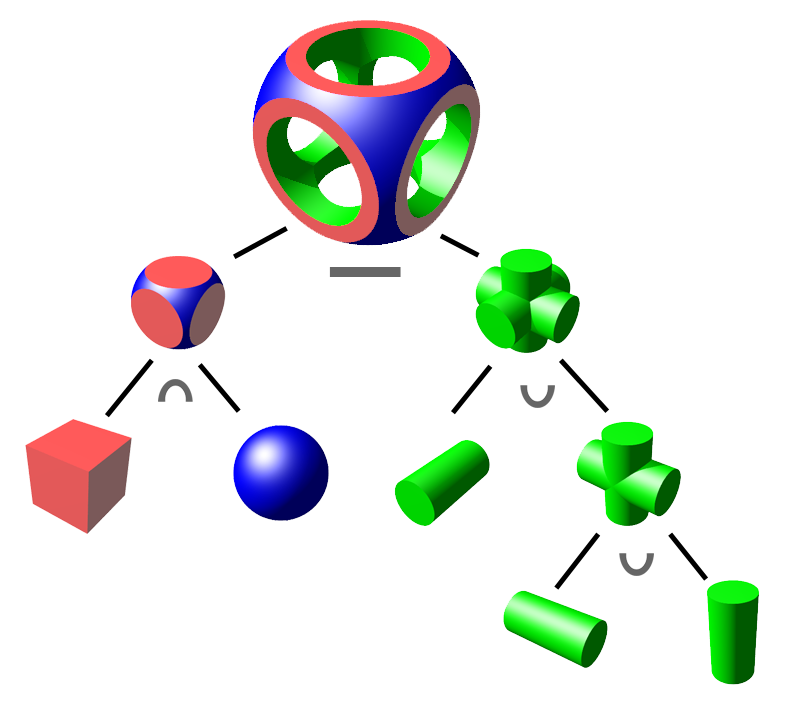
\includegraphics[width=0.5\textwidth]{Pictures/Csg_tree.png}
\caption{CSG object tree}
\label{fig:csg_tree}
\end{figure}
One way of representing a geometry in CAD is the approach of \emph{constructive solid geometry} (short: CSG). The basic idea is to start from a set of primitives, e.g. a sphere, cylinder and cube. Basic Boolean operations link these primitives towards a complex geometry. This procedure can be seen in figure \ref{fig:csg_tree}.

Key advantages of this format is the precise representation using very few storage memory. However, not all desired forms can be represented by CSG and hence, a second type of geometry description is needed. 
\subsubsection{Boundary representation}
A different kind of modelling approach is the so-called \emph{boundary representation}. Instead of storing the geometry information at every single point, \emph{BREP} formats only save the boundary surface of the body. The interior is assumed to be uniformly filled. Especially in big geometries this approach simplifies the model immensely to an extend that amounts of data are better to handle. Surfaces can be stored as tetrahedrons (see later STL files) or in NURBS patches.
Furthermore, holes in the body are possible by saving the surface normal of the boundary surface. 

By the boundary representation arbitrary geometries can be created. Data amounts to fulfill a certain precision are larger than by the csg representation, but BREP files are usually easier to work with. Beware, that unreal geometries can be created using BREP formats.
\subsection{Data exchange file formats}
